\documentclass{report}

\usepackage{graphicx}
\usepackage{titlesec}

\begin{document}
	\begin{titlepage}
		\centering
		
\includegraphics[scale=0.3]{logo_universitas.png}
		{\bfseries\Large
			Universitas Pradita\\
		 	Teknik Informatika\\
			\vskip2cm
			Mikrokernel Arsitektur\\
		}
		\vskip2cm
		{\bfseries\Large
			Nama Penulis:\\
		}
		\vskip0.5cm
		{\bfseries
		1. Paris Matio\\
		2. Bryant Elmer\\
		3. Richard Haryono Yang
		}
			
		\vfill
		{\large
			27 Maret 2023\\
		}
	\end{titlepage}
	
	\title{{\Huge Mikrokernel Architecture}}

	\chapter*{Apa itu kernel?}
	Kernel adalah bagian inti dari sistem operasi yang mengelola sumber daya. 
	
	\begin{enumerate}
	
	\item Itu juga bertindak sebagai jembatan antara perangkat lunak dan perangkat keras. 
	
	\item Ini adalah salah satu program pertama yang dijalankan setelah Boot-loader.
	
	\item Ini mengelola berbagai layanan seperti manajemen input dan output, menangani berbagai panggilan sistem, dan sebagainya. Selain itu, kernel berada pada tingkat abstraksi yang rendah.
	
	\item Kernel juga bertugas menyediakan berbagai program dengan akses aman ke perangkat keras mesin. 
	
	\item Ini juga menentukan kapan dan berapa lama aplikasi tertentu akan menggunakan perangkat keras tertentu.
	
	\end{enumerate}	

	\vskip0.5cm

	\section*{Tipe Kernel}
	
	Ada dua jenis kernel:
	
	1. Mikrokernel
	
	2. Kernel monolitik
	
	\vskip0.5cm
	
	\subsection*{1. Mikrokernel}
	
	Mikrokernel adalah perangkat lunak atau program yang berisi layanan pengguna dan kernel di ruang alamat yang terpisah. Karena ukuran Mikrokernel lebih kecil dari kernel Monolitik. Karena layanan pengguna dan layanan kernel berada di ruang alamat yang berbeda, untuk tujuan komunikasi, pengiriman pesan digunakan, yang membuat eksekusi mikrokernel menjadi lebih lambat.
	
	Meskipun demikian, mikrokernel mudah diperpanjang. Akibatnya, jika layanan baru perlu ditambahkan, tidak diperlukan perubahan pada kernel. Selanjutnya, jika layanan pengguna gagal, itu tidak berpengaruh pada pengoperasian mikrokernel.
	
	Mari kita bahas beberapa poin lagi untuk memahami mikrokernel dengan cara yang lebih baik: 
	
	\begin{enumerate}
		\item Ini hanya menyediakan memori minimal dan layanan manajemen proses.
		
		\item Mikrokernel dan lingkungan penggunanya biasanya ditulis dalam bahasa pemrograman C++ atau C, dengan sedikit rakitan yang disertakan untuk ukuran yang baik. Namun, bahasa implementasi lainnya dimungkinkan dengan beberapa pengkodean tingkat tinggi.
		
		\item Contoh mikrokernel antara lain QNX, Minix, Symbian, Mac OS X, L4Linux, Integrity, K42, dan lain sebagainya.
	\end{enumerate}

	\vskip0.5cm
	
	\subsection*{2. Kernel Monolitik}
	Kernel monolitik adalah program atau perangkat lunak di mana kernel dan layanan pengguna berbagi ruang alamat yang sama. Panggilan sistem digunakan agar layanan pengguna menggunakan layanan kernel apa pun. Ini memungkinkan kernel monolitik untuk mengeksekusi lebih cepat daripada mikrokernel.
	
	Selain itu, kernel monolitik berukuran jauh lebih besar daripada mikrokernel. Karena layanan pengguna dan kernel hadir di ruang alamat yang sama, kernel monolitik sulit untuk diperluas. Akibatnya, untuk menambahkan layanan apa pun, perubahan harus dilakukan pada seluruh kernel.
	
	Namun, kerugian utama dari kernel monolitik adalah jika layanan pengguna gagal, seluruh sistem mungkin gagal.
	
	\begin{enumerate}
		\item Dalam ruang kernel, kernel monolitik mengelola semua layanan sistem dasar seperti manajemen proses, manajemen memori, komunikasi I/O, penanganan interupsi, sistem file, dan seterusnya.
		
		\item Dalam jenis pendekatan Kernel ini, seluruh sistem operasi berjalan dalam mode kernel sebagai satu program. Sistem operasi terdiri dari prosedur yang dihubungkan bersama untuk membentuk program biner besar yang dapat dieksekusi.
		
		\item Contoh kernel monolitik adalah Microsoft Windows, Linux, BSD (OpenBSD, NetBSD, FreeBSD), Solaris, DOS, OpenVMS, dll.
	\end{enumerate}

	\vskip0.5cm

	\section*{Arsitektur Mikrokernel}

	\begin{figure}
		\centering
		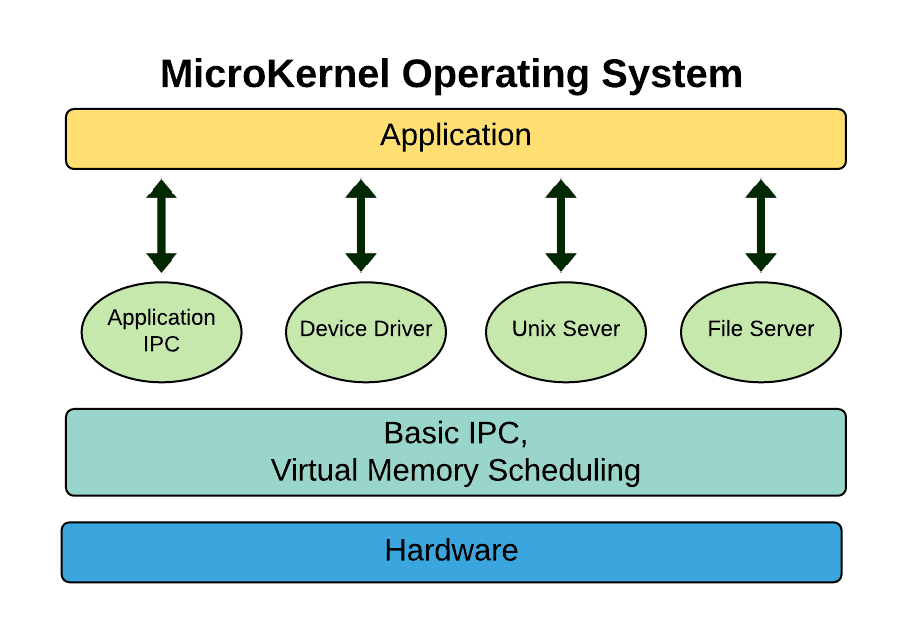
\includegraphics[width=12cm]{Mikrokernel-1.png}
		\caption{Mikrokernel Operating System}
	\end{figure}
	
	Mikrokernel adalah komponen paling penting dalam pengoperasian sistem operasi yang tepat. Mikrokernel melakukan fungsi dasar seperti manajemen memori, algoritma penjadwalan proses, dan komunikasi antar proses.
	
	Pada gambar di atas, Algoritma penjadwalan proses, memori, dan komunikasi antarproses semuanya disertakan. Ini adalah satu-satunya program yang berjalan pada mode istimewa, yaitu mode kernel. Fungsi OS lainnya dipindahkan dari mode kernel dan dijalankan dalam mode pengguna. Driver perangkat, aplikasi, server file, komunikasi antarproses, dan seterusnya adalah contoh dari fungsionalitas ini.
	
	Selain itu, kernel bertanggung jawab atas layanan penting karena merupakan komponen OS yang paling penting. Akibatnya, hanya layanan terpenting yang ada di dalam kernel di bawah desain ini. Layanan sistem operasi lainnya, di sisi lain, termasuk dalam perangkat lunak aplikasi sistem.
	
	Mikrokernel sepenuhnya bertanggung jawab atas layanan terpenting sistem operasi, yaitu sebagai berikut:
	
	\begin{figure}
		\centering
		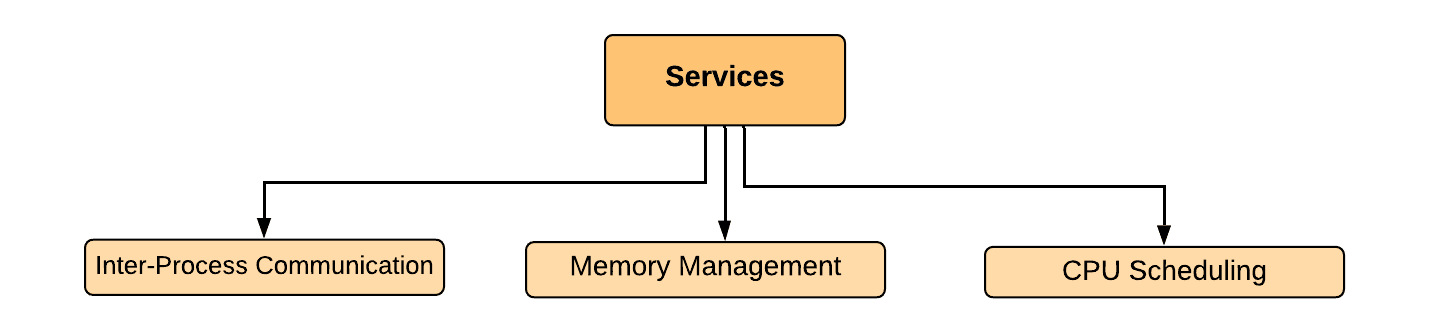
\includegraphics[width=12cm]{Mikrokernel-2.png}
		\caption{The Structure of the system services}
	\end{figure}
	
	\subsection*{Inter-Process Communication}
	
	Interaksi proses disebut sebagai komunikasi antarproses. Ada beberapa utas dalam suatu proses. Utas dari proses apa pun berinteraksi satu sama lain di ruang kernel. Pesan dikirim dan diterima melalui port di seluruh utas. Ada beberapa port di tingkat kernel, termasuk port proses, port luar biasa, port bootstrap, dan port terdaftar. Semua port ini berinteraksi dengan proses ruang pengguna.
	
	\subsection*{Memory Management}
	
	Manajemen memori menetapkan ruang di memori utama dan untuk mengelola operasi yang berbeda antara disk dan memori utama. Namun, ada juga pembuatan memori virtual untuk proses. Memori virtual berarti bahwa jika suatu proses memiliki ukuran lebih besar dari memori utama, itu dipartisi menjadi beberapa bagian dan disimpan. Setelah itu, setiap bagian dari proses tersebut disimpan di dalam memori utama satu per satu hingga CPU mengeksekusinya.
	
	\subsection*{CPU Scheduling}
	
	CPU SCHEDULING adalah proses untuk menentukan proses mana yang akan berjalan selanjutnya di CPU dan proses mana yang akan di-HOLD sementara yang lain sedang berjalan. Semua proses antri dan dijalankan secara berurutan. Setiap proses memiliki tingkat prioritas, dan prosedur prioritas tertinggi dilakukan terlebih dahulu. Penjadwalan CPU dapat membantu Anda mendapatkan hasil maksimal dari komputer Anda. Selain itu, sumber daya digunakan secara lebih efektif. Ini juga mengurangi jumlah waktu yang dihabiskan untuk menunggu.
	
	\vskip0.5cm
	
	\section*{Fungsi Mikrokernel}
	\begin{enumerate}
		\item Memisahkan komponen inti dari sistem operasi menjadi modul-modul yang lebih kecil dan independen, seperti pengelolaan memori, sistem file, dan jaringan.
		
		\item Memungkinkan pengembang untuk dengan mudah menambahkan dan mengubah fungsi sistem operasi tanpa mempengaruhi fungsi lainnya.
		
		\item Mengoptimalkan skalabilitas sistem operasi sehingga dapat disesuaikan dengan kebutuhan dan ukuran yang berbeda.
		
		\item Memungkinkan sistem operasi lebih modular sehingga memungkinkan pengembang untuk lebih mudah menguji dan memodifikasi komponen sistem operasi.
		
		\item Meningkatkan keamanan sistem operasi dengan menjalankan fungsi inti yang kritis dalam ruang kernel yang terisolasi dari aplikasi lainnya, sehingga mencegah kesalahan kernel mempengaruhi aplikasi lainnya.
		
		\item Memungkinkan sistem operasi lebih mudah dipindahkan ke platform yang berbeda karena fungsi inti yang kritis dijalankan dalam ruang kernel yang terisolasi dari hardware.
		
		\item Meningkatkan efisiensi sistem operasi dengan mengurangi overhead dan mempercepat waktu respon sistem operasi.
		
		\item Memungkinkan sistem operasi untuk lebih mudah dikembangkan dan dipelihara dengan menjaga modul-modul yang berbeda terpisah satu sama lain.
		
		\item Meningkatkan fleksibilitas dan adaptabilitas sistem operasi dengan memungkinkan pengembang untuk memperluas atau mengubah fungsionalitas sistem operasi tanpa mempengaruhi komponen inti yang lain.
		
		\item Menyediakan lingkungan yang lebih terstruktur bagi pengembang dan peneliti sistem operasi untuk menguji, mengevaluasi, dan memodifikasi sistem operasi.
	\end{enumerate}

	\vskip0.5cm
	
	\section*{Kelebihan Mikrokernel}
	
	\begin{enumerate}
		\item Karena arsitektur Mikrokernel kompak dan terisolasi, ia dapat bekerja lebih baik.
		
		\item Mikrokernel aman karena hanya komponen yang disediakan yang akan mengganggu fungsionalitas sistem. 
		
		\item Ini mudah diperluas dibandingkan dengan kernel monolitik. 
		
		\item Mikrokernel bersifat modular, dan berbagai modul dapat ditukar, dimuat ulang, dan dimodifikasi tanpa memengaruhi Kernel.
		
		\item Jika dibandingkan dengan sistem monolitik, ada lebih sedikit kerusakan sistem.
		
		\item Antarmuka Mikrokernel membantu implementasi struktur sistem yang lebih modular.
		
		\item Kegagalan server diisolasi dengan cara yang sama seperti kegagalan program pengguna lainnya diisolasi.
		
		\item Karena sistem Mikrokernel serbaguna, berbagai teknik dan API yang diterapkan oleh banyak server dapat hidup berdampingan dalam sistem.
		
		\item Saat keamanan dan stabilitas meningkat, jumlah kode yang dieksekusi dalam mode kernel berkurang.
		
		\item Ini sangat cocok untuk aplikasi berbasis produk, di mana kami dapat menyediakan produk yang layak minimum (MVP) kepada pelanggan sambil secara bertahap menambahkan lebih banyak rilis dan fitur dengan perubahan minimal.
	\end{enumerate}
	
	\section*{Kekurangan Mikrokernel}
	
	\begin{enumerate}
		\item Dibandingkan dengan sistem monolitik, menyediakan layanan dalam sistem Mikrokernel mahal.
		
		\item Arsitektur ini tidak sesuai untuk sistem yang sering membutuhkan komunikasi dan ketergantungan antar komponen yang berbeda.
		
		\item Sakelar konteks atau pemanggilan fungsi diperlukan saat driver diimplementasikan sebagai prosedur atau proses.
		
		\item Performa sistem Mikrokernel dapat bervariasi, menyebabkan masalah.
	\end{enumerate}
	
\end{document}
